For the managing of the bachelor thesis project different aspects need to be taken into account, like how to do the project in which time and how to ensure a good quality of products. These things are explained in this chapter.

\section{Approach}
The project in general is done in a waterfall model, based on the phases explained in section \ref{sec:phases}. But the internal working of the implementation and testing phase will be done in an agile way due to the fact that the functionalities will be implemented through scenarios, also called use cases.

The usage of an agile way helps to develop a product that fulfill all requirements specified and is maintainable. This happen as a result of the continuous implementation of additional functionalities in existing basic functionalities. 

For the agile way iterations, also called sprints, are planned with one use case, which is selected together with the leader of the department \gls{ds} and one member of the department sales. 

\section{Time Planning}
The project implementation will be done in an agile way, that means for the implementation of the worflow user stories will be created, and they need to be fulfilled. The preparation that needs to be done before are made inside a waterfall model. A general time planning can be seen in table \ref{tab:timeplanning}. 
\begin{table} [h]
	\centering
	\begin{tabular}{|c|c|l|c|} \hline
		\rowcolor{Gray}Phase & Week & Activity & CW \\ \hline
		\multirow{2}{*}{1} & 1-4 & Project planning, Topic introduction & 5-9 \\
		& 4 & Research \gls{es} & 9 \\	\hline	
		Milestone I & 06/03/2018 & Project Plan & 10\\ \hline
		1 & 5,6 & Analysis current state \& requirements & 10-11  \\ \hline
		2 & 7 & Research tools & 12 \\ \hline
		Milestone II & 27/03/2018 & Midterm report & 13\\ \hline
		2 & 9 & Research tools & 13 \\ \hline
		Milestone III & ? & Midterm presentation & ? \\ \hline
		\multirow{2}{*}{3} & 10,11 & Designing new workflow & 14-15 \\
		& 12 & Testing design & 16 \\ \hline
		\multirow{2}{*}{4} & 13-17 & Implementing worflow & 17-21 \\
		& 18 & Testing workflow & 22 \\ \hline
		5 & 19 & Final preparation of report \& presentation & 23 \\ \hline
		Milestone IV & 12/06/2018 & Final Report & 24\\ \hline
		Milestone V & ? & Final presentation & ? \\ \hline
	\end{tabular}
	\caption{Time planning of project}
	\label{tab:timeplanning}
\end{table}

\section{Quality Assurance}
The project consist out of three major deliverable categories that have different quality approaches. They are listed below:
\begin{enumerate}
	\item Documents: \newline
	To create qualitatively high documents two techniques are used. On the one hand the writing is done with a tool that checks the orthographic and the grammar and on the other one is the document reviewed by other persons to check the logic and understandability. 
	\item Diagrams: \newline
	In the analysis and the design phase diagrams need to be created. First of all the used diagram types have defined standards, these standards must be fulfilled. Therefore, exists tools that can handle the checking. This will be used. Additional the logic will be checked by persons that currently work (or will work) in the processes visualized in the diagram. 
	\item Implementation: \newline
	For the implementation different use cases will be created, that need to be implemented. The checking will be that they can be executed without errors. Furthermore, if code is created, it will be done based on the defined standard of the used programming language and test driven.
\end{enumerate}
The created results will be regular presented and discussed with involved persons. That leads to the possibility to avoid big problems, cause of their early detection.

\section{Deliverables}
At the end of the internship a working process should be implemented. That also needs to be documented in the sense that other developer can maintain the implemented process. Also a user manual should be created for the user of the process.

\section{Risk Management}
Inside this section already find risks will be presented in the figure \ref{fig:risks}. They could be changed through the time, cause of currently unknown situations.
%\newpage
%\begin{figure}[h]
%	\begin{center}
%		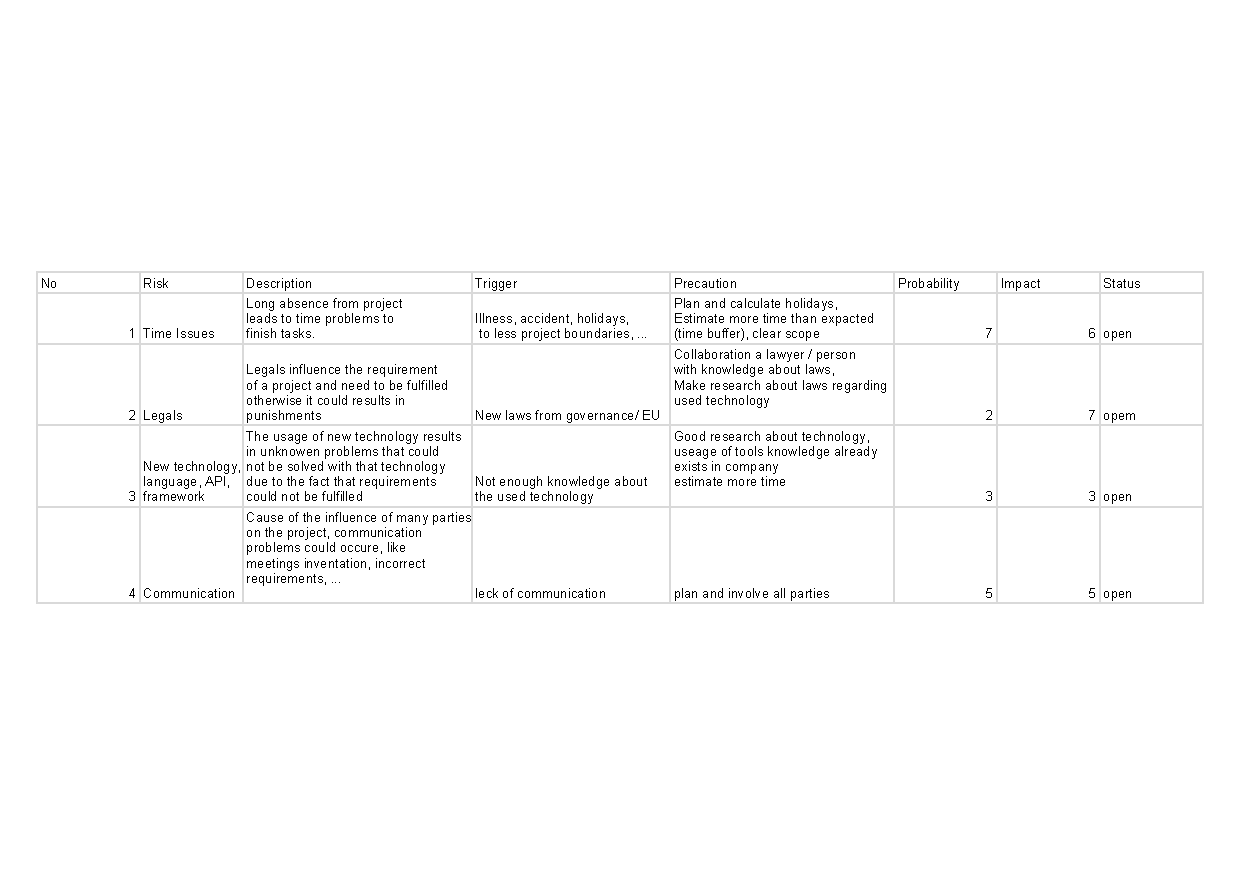
\includegraphics[width=0.9\textheight,angle=90]{./mgnt/risks.pdf}
%		\caption{Figure Risk Management}
%		\label{fig:risks}
%	\end{center}
%\end{figure}
